%% ===============================
%%  BEXT white paper
%%  (September 2014)
%% ===============================

%% Document options
\documentclass[a4paper,11pt]{report}
\usepackage[a4paper]{geometry}
\usepackage{graphicx,rotating}
\usepackage{cite}
\usepackage{amssymb}
\usepackage{mathrsfs}
\usepackage{amsmath}
\usepackage{amsfonts}
\usepackage{multirow}
\usepackage{eurosym}
\usepackage{dcolumn}
\usepackage[pagewise]{lineno}
\usepackage{lscape}
\usepackage{url}

%% Hack to make math formulas bold in section titles
\makeatletter
\DeclareRobustCommand*{\bfseries}{%
  \not@math@alphabet\bfseries\mathbf
  \fontseries\bfdefault\selectfont
  \boldmath
}
\makeatother

%% Some definitions 
%%%%%
\newcommand{\bbonu}{\ensuremath{\beta\beta0\nu}}
\newcommand{\bbtnu}{\ensuremath{\beta\beta2\nu}}
\newcommand{\qbb}{\ensuremath{Q_{\beta\beta}}}
\newcommand{\Qbb}{\ensuremath{Q_{\beta\beta}}}
%\newcommand{\mbb}{\ensuremath{\langle m_{\nu} \rangle}}
\newcommand{\mbb}{\ensuremath{m_{\beta\beta}}}
\newcommand{\mbba}{\ensuremath{m_{\beta\beta}^a}}
\newcommand{\mbbb}{\ensuremath{m_{\beta\beta}^b}}
\newcommand{\mbbt}{\ensuremath{m_{\beta\beta}^t}}

\newcommand{\kgy}{\ensuremath{\rm kg \cdot y}}
\newcommand{\ckky}{\ensuremath{\rm counts/(keV \cdot kg \cdot y)}}

\newcommand{\bb}{\ensuremath{\beta\beta}}
\newcommand{\Tonu}{\ensuremath{T^{0\nu}_{1/2}}}
\newcommand{\Ttnu}{\ensuremath{T^{2\nu}_{1/2}}}
\newcommand{\MO}{\ensuremath{{}^{100}{\rm Mo}}}
\newcommand{\SE}{\ensuremath{{}^{82}{\rm Se}}}
\newcommand{\ND}{\ensuremath{{}^{150}{\rm Nd}}}
\newcommand{\XE}{\ensuremath{{}^{136}\rm Xe}}
\newcommand{\BA}{\ensuremath{{}^{136}\rm Ba}}
\newcommand{\CS}{\ensuremath{{}^{137}\rm Cs}}
\newcommand{\GE}{\ensuremath{{}^{76}\rm Ge}}
\newcommand{\TE}{\ensuremath{{}^{128}\rm Te}}
\newcommand{\TEX}{\ensuremath{{}^{130}\rm Te}}
\newcommand{\TL}{\ensuremath{{}^{208}\rm{Tl}}}
\newcommand{\CA}{\ensuremath{{}^{48}\rm Ca}}
\newcommand{\PO}{\ensuremath{{}^{214\rm Po}}}
\newcommand{\U}{\ensuremath{{}^{235}\rm U}}
\newcommand{\CO}{\ensuremath{{}^{60}\rm Co}}
\newcommand{\CD}{\ensuremath{^{116}{\rm Cd}}}
\newcommand{\AM}{\ensuremath{^{241}{\rm Am}}}
\newcommand{\THO}{\ensuremath{{}^{232}{\rm Th}}}
\newcommand{\BI}{\ensuremath{{}^{214}}Bi}
\newcommand{\RN}{\ensuremath{{}^{222}}Rn}
\newcommand{\Monu}{\ensuremath{\Big|M^{0\nu}\Big|}}
\newcommand{\Mtnu}{\ensuremath{\Big|M^{2\nu}\Big|}}
\newcommand{\Gonu}{\ensuremath{G^{0\nu}(E_0, Z)}}
\newcommand{\Gtnu}{\ensuremath{G^{2\nu}(E_0, Z)}}
\newcommand{\FT}{\ensuremath{40 \ \textrm{mg/cm}^2}} 
\newcommand{\FTtwe}{\ensuremath{20 \ \textrm{mg/cm}^2}} 
\newcommand{\FTeig}{\ensuremath{80 \ \textrm{mg/cm}^2}} 
\newcommand{\tetaot}{\ensuremath{\theta_{13}}}
\newcommand{\tetatt}{\ensuremath{\theta_{23}}}
\newcommand{\tetaotw}{\ensuremath{\theta_{12}}}
\newcommand{\deltt}{\ensuremath{\Delta_{23}}}
\newcommand{\delot}{\ensuremath{\Delta_{13}}}
\newcommand{\dsun}{\ensuremath{\Delta_{\rm sun}^2}}
\newcommand{\datm}{\ensuremath{\Delta_{\rm atm}^2}}
\newcommand{\Toh}{\ensuremath{T_{1/2}}}
\newcommand{\M}{\ensuremath{M}}
\newcommand{\W}{\ensuremath{W}}
\newcommand{\GA}{\ensuremath{g_A}}
\newcommand{\NA}{\ensuremath{N_A}}
\newcommand{\wbbo}{\ensuremath{N_{\beta\beta}^{0\nu}}}
\newcommand{\wbbt}{\ensuremath{N_{\beta\beta}^{2\nu}}}
\newcommand{\wupper}{\ensuremath{N_{upper}^{2\nu}}}
\newcommand{\epst}{\ensuremath{\epsilon_{\beta\beta}}}
\newcommand{\epsa}{\ensuremath{\epsilon_{\beta\beta}^{\rm accep}}}
\newcommand{\epsr}{\ensuremath{\epsilon_{\beta\beta}^{\rm rec}}}
\newcommand{\epss}{\ensuremath{\epsilon_{\beta\beta}^{\rm sel}}}
\newcommand{\TO}{\ensuremath{T_{1/2}^{0\nu}}}
\newcommand{\TT}{\ensuremath{T_{1/2}^{2\nu}}}
\newcommand{\ev}{\ensuremath{\rm eV}} 
\newcommand{\mev}{\ensuremath{\rm meV}} 
\newcommand{\Mev}{\ensuremath{\rm MeV}} 
\newcommand{\Kev}{\ensuremath{\rm KeV}} 
\newcommand{\mm}{\ensuremath{mm}} 
\newcommand{\cm}{\ensuremath{cm}} 
\newcommand{\kg}{\ensuremath{kg}}  
\newcommand{\ubq}{\ensuremath{\mu Bq / kg}} 
\newcommand{\sn}{SuperNEMO} 

%%%
% Some handy commands

\newcommand{\Xe}{\ensuremath{^{136}}Xe}

% Bi-214
\newcommand{\Bi}{\ensuremath{^{214}}Bi}

% Tl-208
\newcommand{\Tl}{\ensuremath{^{208}}Tl}

% Pb-208
\newcommand{\Pb}{\ensuremath{^{208}}Pb}

% Po-214
\newcommand{\Po}{\ensuremath{^{214}}Po}

\newcommand{\GES}{\ensuremath{{}^{68}\rm Ge}}

% bru
\newcommand{\bru}{cts/(keV$\cdot$kg$\cdot$y)}

% Saltos de carro en tablas
\newcommand{\minitab}[2][l]{\begin{tabular}{#1}#2\end{tabular}}

\def\lpy#1{#1} % use this for final
\def\lpy#1{\Cyan#1\Black} % use this for drafts
\def\lpybox#1{} %% use this for final
\def\lpybox#1{\fbox{\Red{\bf#1}\Black}} % use this for drafts

\def\calE{\mathcal{E}}
\def\Hatom{\textrm{H}$_{\textrm{atom}}$}
\def\Hlight{$\textrm{H}_{\textrm{light}}$}
\def\Hinterac{$\textrm{H}_{\textrm{interac}}$}
\def\waven{cm$^{-1}$}
\def\D{$^2\mathrm{D}_{3/2}$\,}
\def\S{$^2\mathrm{S}_{1/2}$\,}
\def\P{$^2\mathrm{P}_{1/2}$\,}
\def\ns{ns$^{-1}$}

\newcommand{\stwo}{\mbox{$2s\,^3S_1$}}
\newcommand{\p}[1]{\mbox{$3p\,^3P_{#1}$}}
\newcommand{\g}{X$^2$$\Pi$($\nu''=0$)}
\newcommand{\e}{A$^2$$\Sigma^+$($\nu'=0$)}
\newcommand{\gbib}{X$^2$$\Pi$}
\newcommand{\ebib}{A$^2$$\Sigma^+$}


\long\def\symbolfootnote[#1]#2{\begingroup%
\def\thefootnote{\fnsymbol{footnote}}\footnote[#1]{#2}\endgroup}


%% ======================================
\begin{document}

%% Title page and abstract
\begin{titlepage}

%%%
\begin{center}
{\large \sf WHITE PAPER} \\ \vspace{0.65cm}
{\Huge \bf Towards a Barium Experiment in a Xenon TPC (BEXT)} \\ \vspace{0.75cm}
{(16 May 2011)} \\ \vspace{0.35cm}
\end{center}
%%%

\begin{center}
\begin{minipage}{15cm}
\section{Introduction}
We outline in this paper the theoretical basis and our proposed experimental roadmap to study the feasibility of tagging the single barium ion produced in the  \bb\ decay of \XE. The possibility of resonant excitation of the barium ion to its first excited state using lasers of suitable wavelength and the subsequent observation ``tagging" of the emitted fluorescence was proposed by XXX and has been actively pursued, for more than XXX years by members of the EXO collaboration, which have conducted a very active R\&D, considering tagging both in liquid and gaseous xenon TPCs.  

Both EXO and its proposed continuation, NEXO, are liquid xenon TPCs (LXe). The NEXT collaboration, on the other hand, is currently building the NEXT-100 detector, a high pressure xenon TPC (HPXe) using electroluminescence to amplify the ionisation signal. The R\&D phase of NEXT, already completed, has shown excellent energy resolution and the capability of reconstruction of electron tracks. 

Barium tagging in LXe and HPXe are two different problems. The R\&D of EXO has been focused on extracting the barium ion, either using a probe (in the LXe) detector, or a dynamic electric field to guide the ion outside a gas TPC. In both cases, the idea is to confine the barium ion in a magneto trap in vacuum, before shining the lasers. The rational behind this approach is clear: in situ tagging, even it one demonstrates that is possible, would be, in any case, difficult. It would require good and fast location of the ion, a reliable laser guiding system, and sophisticated instrumentation. On the other hand it may turn out that extracting the ion from the chamber is an even more formidable problem. 

The authors of this paper are members of the NEXT collaboration and of the CLPU. Our goal is to outline the theoretical basis and the experimental roadmap to establish if barium tagging in situ in a HPXE TPC if possible.  

\end{minipage}
\end{center}

\begin{center}
\pagebreak 

{\LARGE \bf The BEXT collaboration}

\vspace{0.4cm}

{\small \sc . Peralta Conde\symbolfootnote[1]{Contact email: aperalta@clpu.es}, J. Api\~naniz, E. Garc\'ia,  M. Rico, C. Salgado, M. S\'anchez, F. Valle, A. Vazquez, and L. Roso}\\
{\it Centro de L\'aseres Pulsados, CLPU, Parque Cient\'ifico, E-37185 Villamayor, Salamanca, Spain.}

\vspace{0.3cm}

{\small \sc  J.J.~G\'omez-Cadenas\symbolfootnote[1]{Contact email: gomez@mail.cern.ch}, P. Ferrario, D. Gonz\'alez, A. Goldschmidt N.~L\'opez-March,  \\I.~Liubarsky, D. Nygren, F.~Monrabal, A. ~Simó}\\
{\it Instituto de F\'isica Corpuscular (IFIC), CSIC \& Univ.\ de Valencia, Valencia, Spain}

\end{center}




\end{titlepage}


%% Contents
\tableofcontents

%% CHAPTER 1. THE PHYSICS %%%%%%%%%%%%%%%
\chapter{\bbonu\ experiments and barium tagging}

\section{Introduction}

\begin{itemize}
\item General context
\item NEXT description
\item BaTa for NEXT
\item Mention in situ BaTa and "out situ" BaTa?
\end{itemize}



%
%
%%% CHAPTER 2. EASY AND SOFT %%%%%%%%%%%%%
\chapter{Barium laser spectroscopy}



\section{Barium Tagging}\label{BaTa}

The first question that needs to be addressed is the choice of system for the tagging process. Although it seems obvious to explore the possibility of barium tagging (BaTa) in doubly ionized Ba, an inspection of the doubly ionized barium energy levels discards this possibility.  According to \cite{Sansonetti10} the first excited state of Ba$^{++}$ lies at 132770.79\,\waven which corresponds to an energy of 16.46\,eV, or equivalently to a radiation of around 75\,nm wavelength. Any radiation below 200\,nm, i.e., vacuum ultraviolet (VUV) or extreme ultraviolet (XUV), is not easily accesible and its generation and handling involves major experimental difficulties. As a consequence, the tagging process must take place in singly ionized Ba, and accordingly the recombination process Ba$^{++}\rightarrow$Ba$^{+}$ must be somehow stimulated. We will discuss this in detail in further sections. 

\begin{figure}[ht!]
\begin{center}
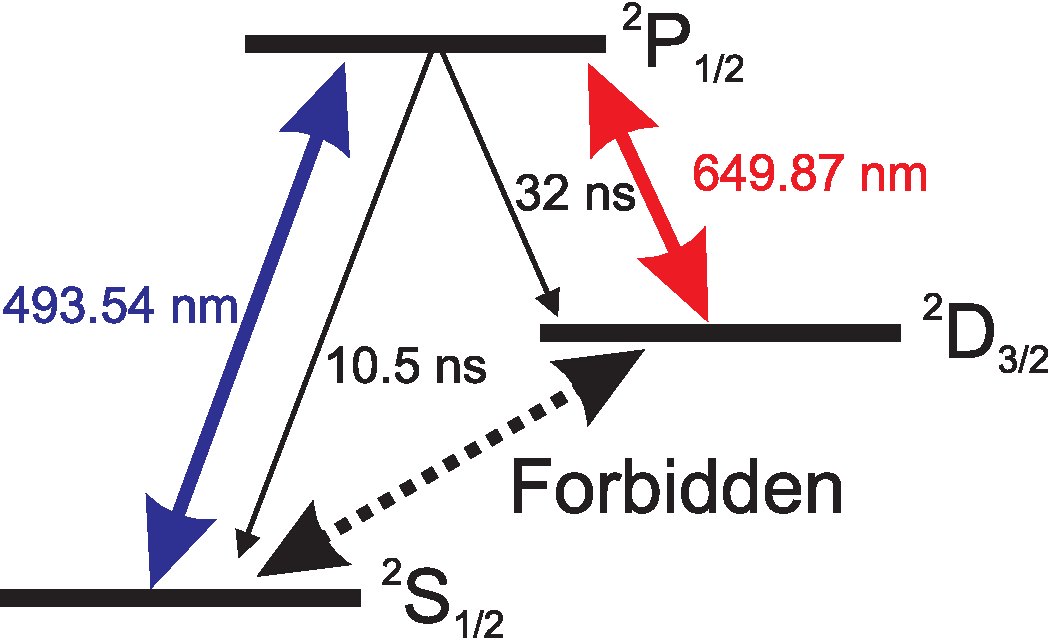
\includegraphics[width=8.3cm, height=5cm]{imgs/levelscheme.pdf}
\caption{\label{levelscheme} Level scheme of the three lowest states of Ba$^+$ ions and the corresponding radiative lifetimes. The notation corresponds to $^{2\mathrm{S}+1}\mathrm{L}_\mathrm{J}$ being S the spin angular momentum, L the angular momentum, and J=L+S.}
\end{center}
\end{figure}

Figure\,\ref{levelscheme} shows the first three states of Ba$^+$ ions together with the corresponding radiative lifetimes. The level structure of Ba$^+$ is somehow peculiar because the first excited state, i.e., the D state, is not optically accesible considering the dipole approximation and single photon transitions, from the ground state.  The selection rules for $\pi$ polarized light are: $ \Delta\mathrm{L}=1, \,\Delta\mathrm{S}=0, \,\Delta\mathrm{J}=0,\pm1, \,\Delta m_\mathrm{J}=0\,(\text{with forbidden}\, \Delta\mathrm{J}=0;\,\mathrm{m_J}=0\rightarrow\mathrm{m'_J}=0)$.  According to this, the state D is metastable with a radiative lifetime of the order of around 80\,s \textbf{[pod\'eis dar la referencia de este dato???]}. 

A possible scheme for the tagging process would involve laser pumping of the S$\rightarrow$P transition, and the collection of the fluorescence of the P$\rightarrow$D one. Since excitation and fluorescence wavelengths are very different, they can be efficiently discriminated using filters which simplifies enormously the detection systems. Because the D state is metastable, that scheme makes necessary to repump the population driven to this state to the S or P states in order to obtain an appreciable fluorescence signal.  We will discuss some possibilities of deshelving the D state below. 

The population dynamics is ruled by the time dependent Schr\"odinger equation 
\begin{equation}
\label{Schr}
 i\hbar\frac{\partial\hat{\Psi}(t)}{\partial t}=H(t)\hat{\Psi}(t),
\end{equation}
where $\Psi(t)$ is the statevector of the system and $H(t)$ the
Hamiltonian including the interaction with the laser. If incoherent processes like spontaneous emission need to be taken into account, the Schr\"odinger equation no longer provides an adequate description of the dynamics. For such situations it is necessary to work with density matrix formalism. In this formalism the dynamics is ruled by the so called quantum Liouville equation \cite{Sh90}
\begin{equation}
\label{Density}
 \hbar\frac{\partial\hat{\rho}(t)}{\partial t}=-i\left[H(t), \hat{\rho}(t)\right]
\end{equation}
being $\rho_{ii}$ the population of state i, and $\rho_{ij}$ the coherence between states i an j. In this formalism the relaxation terms $\Gamma$, e.g., ionization, radiative decays or collisional broadening, can be easily taken into account by adding an extra term to Eq.\,\ref{Density}
\begin{equation}
\label{Density}
 \hbar\frac{\partial\hat{\rho}(t)}{\partial t}=-i\left[H(t), \hat{\rho}(t)\right]-\hbar\hat{\Gamma}\hat{\rho}(t).
\end{equation}

\begin{figure}[ht!]
\begin{center}
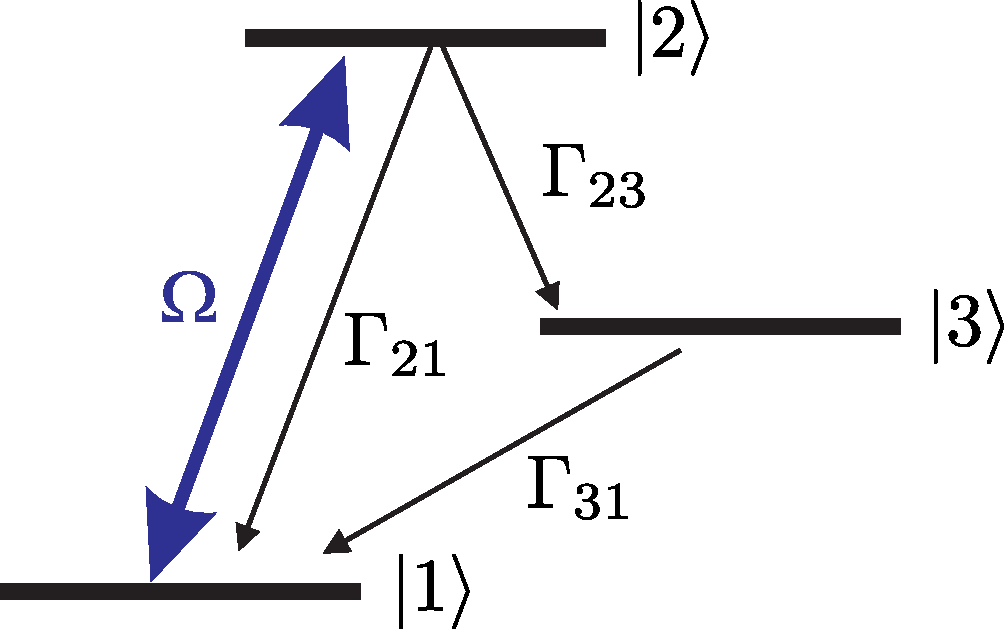
\includegraphics[width=8.3cm, height=5cm]{imgs/levelscheme2.pdf}
\caption{\label{levelscheme2} Level scheme with decay rates. $\Gamma_{ij}=1/\tau_{ij}$.}
\end{center}
\end{figure}

Taking into consideration the system described in Fig.\,\ref{levelscheme} with all the possible decays (see Fig.\,\ref{levelscheme2}), the Hamiltonian that describes the interaction with the laser results in (for simplicity we will assume the laser on resonance with the S$\rightarrow$P transition)
\begin{equation}
H(t)=\frac{1}{2}\left(
\begin{matrix} 
0& \Omega & 0  \\
\Omega & 0 & 0   \\
0 & 0 & 0
\end{matrix}
\right)
\end{equation}
being $\Omega$ the Rabi frequency, i.e., the interaction energy divided by $\hbar$. The population dynamics is described by the following set of differential equations:

\begin{align}
\label{density}
& \rho_{11}'  = -\Omega I\rho_{12}(t) +\Gamma_{21}\rho_{22}(t)+ \Gamma_{31}\rho_{33}  \\ \nonumber
& \rho_{22}'  = \Omega I\rho_{12}-\Gamma_{21}\rho_{22} - \Gamma_{23}\rho_{22}\\  \nonumber
& \rho_{33}'  = \Gamma_{23}\rho_{22}-\Gamma_{31}\rho_{33}\\  \nonumber
& R\rho_{12}'  = - (1/2) R\rho_{12} (\Gamma_{21} +\Gamma_{23} + \Gamma_{31})\\  \nonumber
& I\rho_{12}'  =(1/2)( \Omega (\rho_{11}-\rho_{22}) - I\rho_{12}(\Gamma_{21}+\Gamma_{23}+\Gamma_{31}))\\  \nonumber
& R\rho_{13}'  = (1/2)(\Omega I\rho_{23} -R\rho_{13} (\Gamma_{21}+ \Gamma_{23} + \Gamma_{31}))\\  \nonumber
& I\rho_{13}'  =-(1/ 2)(\Omega R\rho_{23} -I\rho_{13} (\Gamma_{21}+ \Gamma_{23} + \Gamma_{31}))\\  \nonumber
& R\rho_{23}'  = (1/2)( \Omega I\rho_{13} - R\rho_{23} (\Gamma_{21}+ \Gamma_{23} + \Gamma_{31}))\\  \nonumber
& I\rho_{23}'  = -(1/2)( \Omega R\rho_{13}- I\rho_{23} (\Gamma_{21}+ \Gamma_{23} + \Gamma_{31}))
\end{align}
where $\rho_{ii}$ is the population of state $i$, and $R\rho_{ij}$ and $I\rho_{ij}$ are the real and imaginary parts of the coherence between states $i$ and $j$ respectively. It is important to mention that for situations where the decay rates $\Gamma_{ij}$ rule the dynamics of the system, what is called the incoherent limit, i.e., $\Gamma_{ij}\gg\Omega$, the density matrix equations and rate equations are equivalent. Although the latter set of equations is much easier to handle and it is most likely the situation for BaTa, we prefer to have a more general description that will allow us further refinements in the equations, e.g., introduction of different broadening mechanisms as collisional or Doppler broadening. 

For a stationary situation $\rho_{ij}'\rightarrow0$, the population of state 2 reads
\begin{equation}
\label{P2}
P_2=\frac{\Gamma_{31}\Omega^2}{\Gamma_{31}(\Gamma_{21}+\Gamma_{23})(\Gamma_{21}+\Gamma_{31}+\Gamma_{23})+(2\Gamma_{31}+\Gamma_{23})\Omega^2}
\end{equation}
being the rate of red fluorescence photons that need to be detected
\begin{equation}
\label{Photons}
\Gamma_{\text{Photons}}=\Gamma_{23}P_2
\end{equation}

As it was stated above, the rate of fluorescent red photons depends strongly on the decay rate $\Gamma_{31}$ (see Eq.\,\ref{P2}). Since the state D is metastable, it is plausible to think that the relaxation process D$\rightarrow$S will be mediated mainly by collisions. Thus, for the sake of generality we will assume that also collisions affect the decay rate of states S and P. That means:
\begin{align}
\label{Mod_relax}
& \Gamma_{21}^*=\Gamma_{21}+\Gamma_{31}
& \Gamma_{23}^*=\Gamma_{23}+\Gamma_{31}.
\end{align}
In the following we will examine the different limiting cases, dropping the asterisk in the notation of the decay rates for simplicity.

\subsection{Low deshelving rate of state D. $\Gamma_{31}\ll\Gamma_{21}, \Gamma_{23}$}

In this situation the $\Gamma_{Photons}$ is limited by $\Gamma_{31}$
\begin{equation}
\Gamma_{\text{Photons}}\leq\frac{\Gamma_{23}\Gamma_{31}\Omega^2}{\Gamma_{23}\Omega^2}=\Gamma_{31}
\end{equation}
This can be easily understood if one takes into account that the drain of population from D to S states is much slower than the pumping rate from S to P and the natural decays of state P.

\begin{figure}[ht!]
\begin{center}
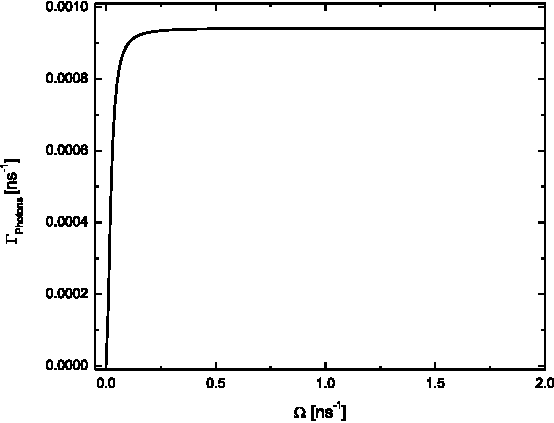
\includegraphics[width=8.3cm, height=6.3cm]{imgs/LowD2D.pdf}
\caption{\label{LowD2D} $\Gamma_{\text{Photons}}$ as a function of the Rabi frequency $\Omega$ for a continuous wave (CW) laser being $\Gamma_{31}=0.001$\ns, $\Gamma_{21}=\frac{1}{10.5}+\Gamma_{31}$\ns, and $\Gamma_{23}=\frac{1}{32}+\Gamma_{31}$\ns. }
\end{center}
\end{figure}

As an example of our discussion, Fig.\,\ref{LowD2D} shows the $\Gamma_{\text{Photons}}$ as a function of the Rabi frequency. It is clear that the rate of red photons is limited by the decay $\Gamma_{31}$.  This can also be seen in Fig.\,\ref{LowDPopu} that shows the population dynamics for $\Omega=1$\ns. Once the population reaches the state D it can not escape in a time scale relevant for the population dynamics. 

\begin{figure}[ht!]
\begin{center}
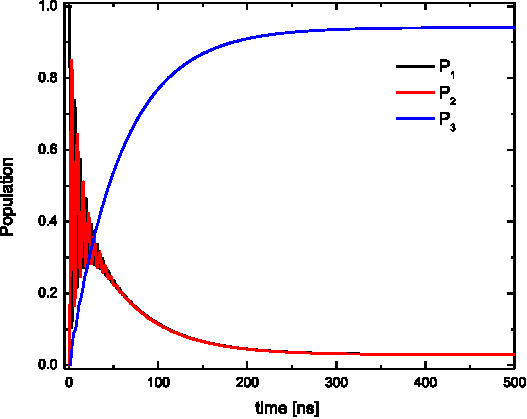
\includegraphics[width=8.3cm, height=6.6cm]{imgs/LowDPopu.pdf}
\caption{\label{LowDPopu} Population dynamics for $\Omega=1$\ns and  $\Gamma_{31}=0.001$\ns.}
\end{center}
\end{figure}
 
At this point it is worth to calculate the saturation intensity, $I_{\text{Saturation}}$, and to give some values that connect theory and experiments. It can be shown \cite{Sh90} that when the Rabi frequency equals the natural decay, the population exhibits Rabi oscillations and the population dynamics is dominated by the laser-matter interaction. In other words, the atomic transition is saturated. Let us assume 
\begin{equation}
\Omega_{\text{Saturation}}\simeq\Gamma_{21}=\frac{1}{10.5}\,\text{ns}^{-1}.
\end{equation}
Taking into account that the Rabi frequency is defined by
\begin{equation}
\Omega=\frac{\mu E}{\hbar}
\end{equation}
being $E$ the laser electric field and $\mu$ the electric dipole moment, and in turn $\mu$ is defined by
\begin{equation}
\mu=\sqrt{\frac{3\epsilon_0 h \lambda_{21}^3}{(2\pi)^2}\frac{1}{\tau_{21}}}
\end{equation}
where $\lambda_{21}$ is the wavelength of the transition, the saturation electric field is
\begin{equation}
E_{\text{Saturation}}=\sqrt{\frac{h2\pi}{3\epsilon_o\tau_{21}\lambda^3}}\simeq350\,\text{V/m}.
\end{equation}
According to this calculation, the required laser intensity for saturating the transition S$\rightarrow$P is
\begin{equation}
I_{\text{Saturation}}=\frac{1}{2}\epsilon_0cE^2_{\text{Saturation}}\simeq0.016\,\text{Wcm}^{-2}.
\end{equation}
Thus, given this value for $I_{\text{Saturation}}$ we can calculate the width of the laser focus for a given laser power. This is critical for NEXT experiment because a wider laser focus will clearly enhance the possibilities of detecting barium atoms. Finally, it is important to notice that the obtained value for the saturation intensity is just a first approximation. When different factors like for example spatial profile of the laser beam or broadening mechanisms of the transition are taken into account, this value tends to be larger. Even so, it is a very useful approximation that directly connects theory and experiments.


\subsection{High deshelving rate of state D. $\Gamma_{31}\gg\Gamma_{21}, \Gamma_{23}$}
\label{HighD}

In this situation
\begin{align}
\label{Mod_relax_large}
& \Gamma_{21}^*\simeq\Gamma_{31}
& \Gamma_{23}^*\simeq\Gamma_{31}.
\end{align}
and accordingly
\begin{equation}
\Gamma_{\text{Photons}}\simeq\frac{\Gamma_{31}\Omega^2}{6\Gamma^2_{31}+3\Omega^2}.
\end{equation}
The maximum $\Gamma_{\text{Photons}}$ will be obtained when $\Omega\gg\Gamma_{31}$, i.e., when the dynamics of the system is ruled by the Rabi frequency:
\begin{equation}
\Gamma_{\text{Photons}}\leq\frac{\Gamma_{31}}{3}.
\end{equation}
Figure\,\ref{2DHighD} shows the $\Gamma_{\text{Photons}}$ as a function of the Rabi frequency, and Fig.\,\ref{popuHighD} the population dynamics for the particular case of $\Omega=1$\,\ns.

\begin{figure}[ht!]
\begin{center}
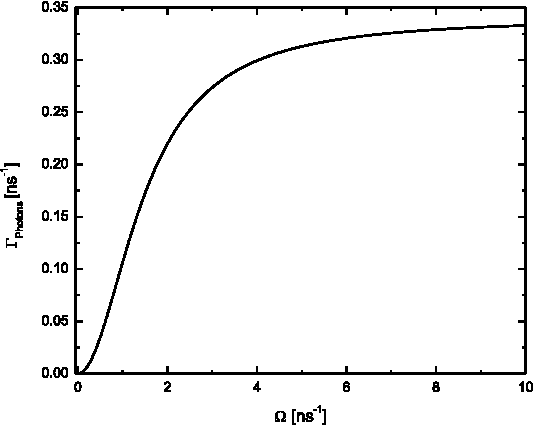
\includegraphics[width=8.3cm, height=6.3cm]{imgs/2DHighD.pdf}
\caption{\label{2DHighD} $\Gamma_{\text{Photons}}$ as a function of the Rabi frequency $\Omega$ for a continuous wave (CW) laser being $\Gamma_{31}=1$\ns, $\Gamma_{21}=\frac{1}{10.5}+\Gamma_{31}$\ns, and $\Gamma_{23}=\frac{1}{32}+\Gamma_{31}$\ns. }
\end{center}
\end{figure}

\begin{figure}[ht!]
\begin{center}
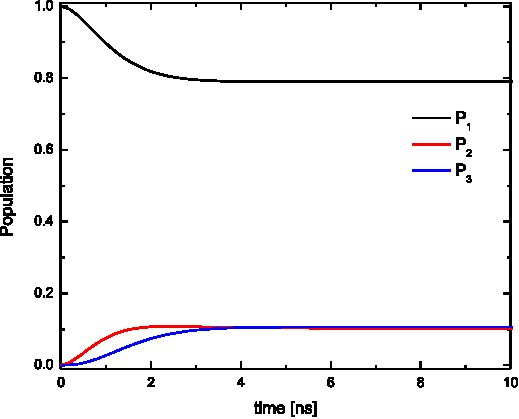
\includegraphics[width=8.3cm, height=6.6cm]{imgs/popuHighD.pdf}
\caption{\label{popuHighD} Population dynamics for $\Omega=1$\ns and  $\Gamma_{31}=1$\ns.}
\end{center}
\end{figure}

\subsection{Medium deshelving rate of state D. $\Gamma_{31}\simeq\Gamma_{21}, \Gamma_{23}$}

In this scenario, and assuming the saturation of the S$\rightarrow$P transition, the rate of red photons that need to be detected reads

\begin{equation}
\Gamma_{\text{Photons}}=\frac{\Gamma_{23}\Gamma_{31}}{2\Gamma_{31}+\Gamma_{23}}.
\end{equation}
This can be clearly seen in Fig.\,\ref{2DMedD} where $\Gamma_{\text{Photons}}$ rapidly saturates as a function of $\Omega$. Figure\,\ref{popuM} shows the population dynamics for the particular situation of $\Omega=1$\ns. 
\begin{figure}[ht!]
\begin{center}
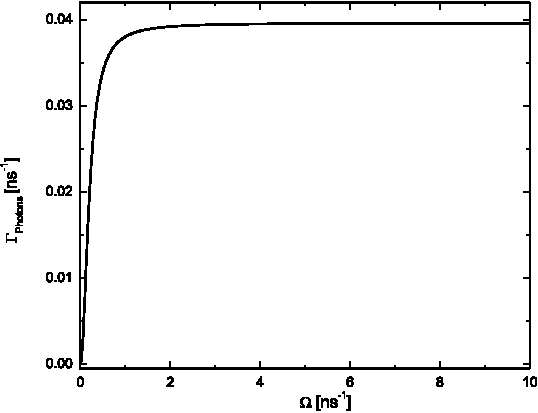
\includegraphics[width=8.3cm, height=6.3cm]{imgs/2DMedD.pdf}
\caption{\label{2DMedD} $\Gamma_{\text{Photons}}$ as a function of the Rabi frequency $\Omega$ for a continuous wave (CW) laser being $\Gamma_{31}=\frac{1}{10}$\ns, $\Gamma_{21}=\frac{1}{10.5}+\Gamma_{31}$\ns, and $\Gamma_{23}=\frac{1}{32}+\Gamma_{31}$\ns}
\end{center}
\end{figure}


\begin{figure}[ht!]
\begin{center}
\includegraphics[width=8.3cm, height=6.6cm]{imgs/popuM.pdf}
\caption{\label{popuM} Population dynamics for $\Omega=1$\ns and  $\Gamma_{31}=\frac{1}{10}$\ns.}
\end{center}
\end{figure}
To summarize this section we plot in Fig.\,\ref{3Dgraph} $\Gamma_{\text{Photons}}$ as a function of $\Omega$ and $\Gamma_{31}$.
\begin{figure}[ht!]
\begin{center}
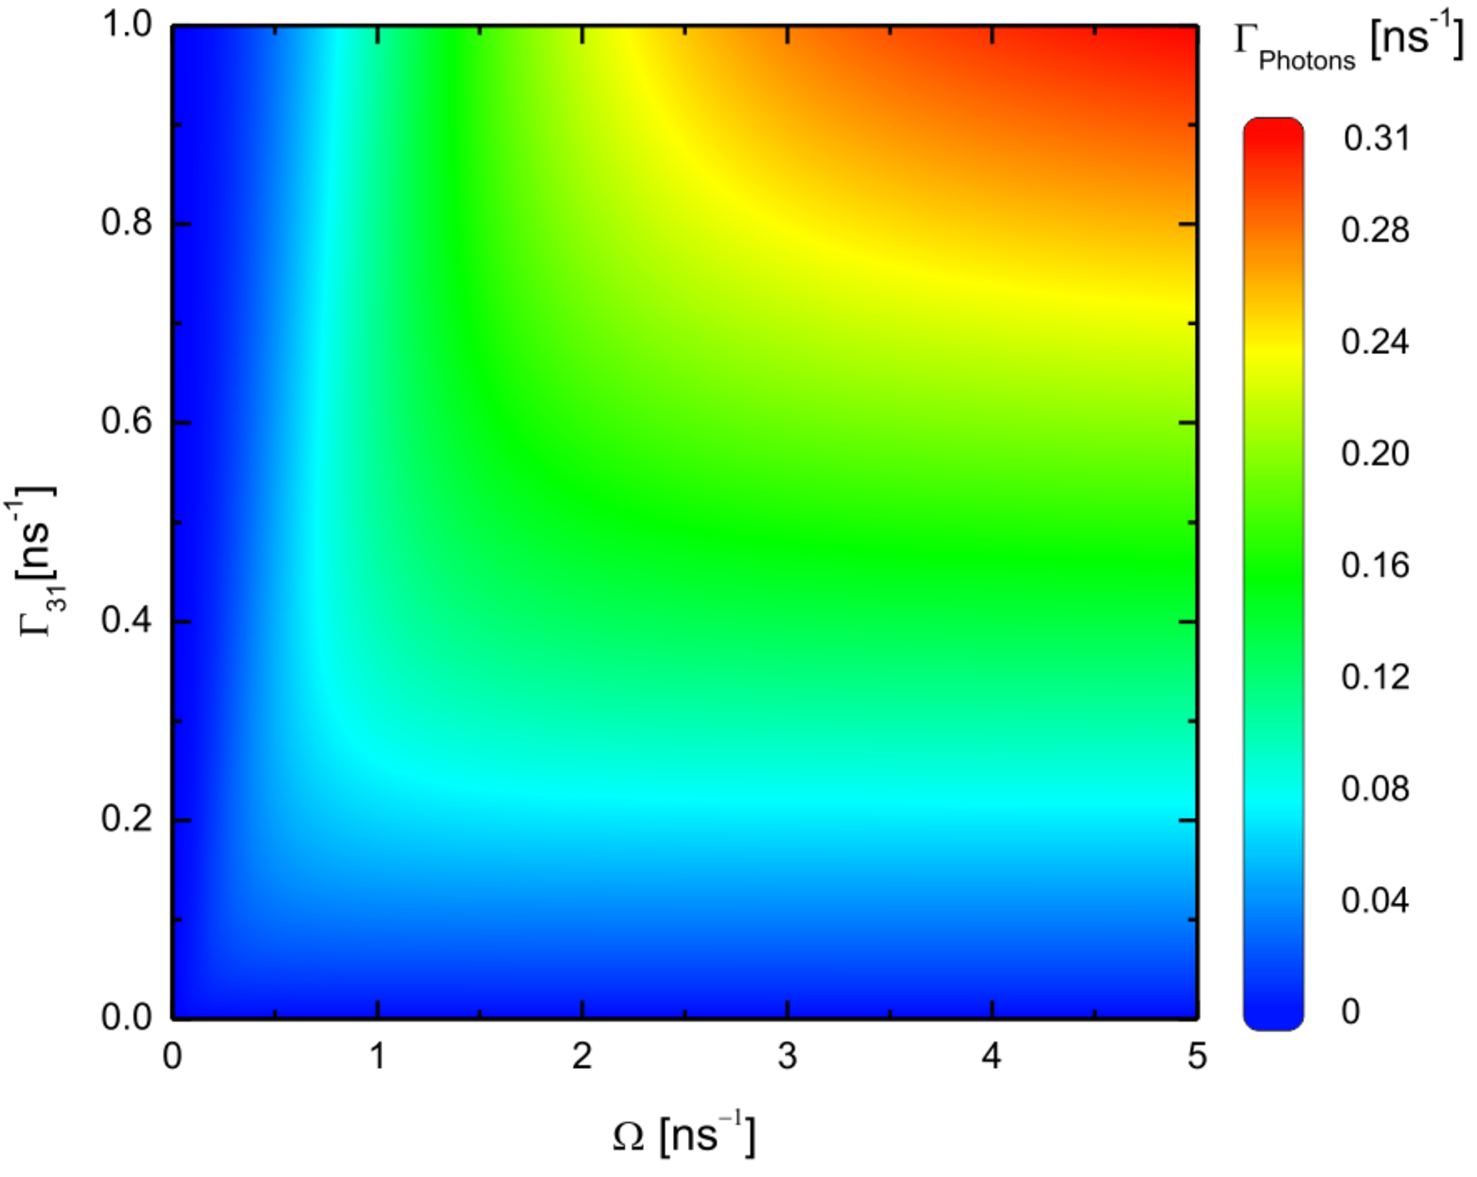
\includegraphics[width=8.3cm, height=6.7cm]{imgs/3Dgraph.pdf}
\caption{\label{3Dgraph} $\Gamma_{\text{Photons}}$ versus $\Omega$ and $\Gamma_{31}$.}
\end{center}
\end{figure}

The description presented here is based on two main assumptions: the recombination process Ba$^{++}\rightarrow$Ba$^+$ is efficient, and there is a mechanism to force the deshelving of the metastable D state. In the following we will describe in detail these premises.

\section{Ba$^{++}\rightarrow$Ba$^+$ recombination}

Aquí habría que mencionar algo de la posible recombinación por aditivos TMA y demás. Efecto en BaTa?

\section{Scattering of the blue laser?}

No estoy seguro si esto merece la pena mencionarlo o no

\section{D state deshelving}

\subsection{Collisions}
\label{Subcol}


As we considered above, collisions can produce not only the deshelving of the D state, but also of other states of the system. The number of collisions in the experimental conditions of NEXT can be estimated using complex models but on one hand it will be far from the scope of this manuscript, and on the other hand according to the results of Section\,\ref{BaTa} it is in principle enough to know the order of magnitude. Thus, we have restricted ourselves to a simple solid sphere model.

Let us suppose that Xe atoms and Ba$^+$ ions behave like solid spheres with diameters d$_1$ and d$_2$ respectively, and occupy a volume V.  We will also assume that the diffusion of Ba$^+$ ions through Xe in the conditions of the NEXT experiment is rather slow, and their velocity is negligible when compared with the velocity of the Xe atoms v$_1$. This approximation is justified by the high pressure of Xe, around 10\,atm, that will be used in NEXT.    

 \begin{figure}[ht!]
\begin{center}
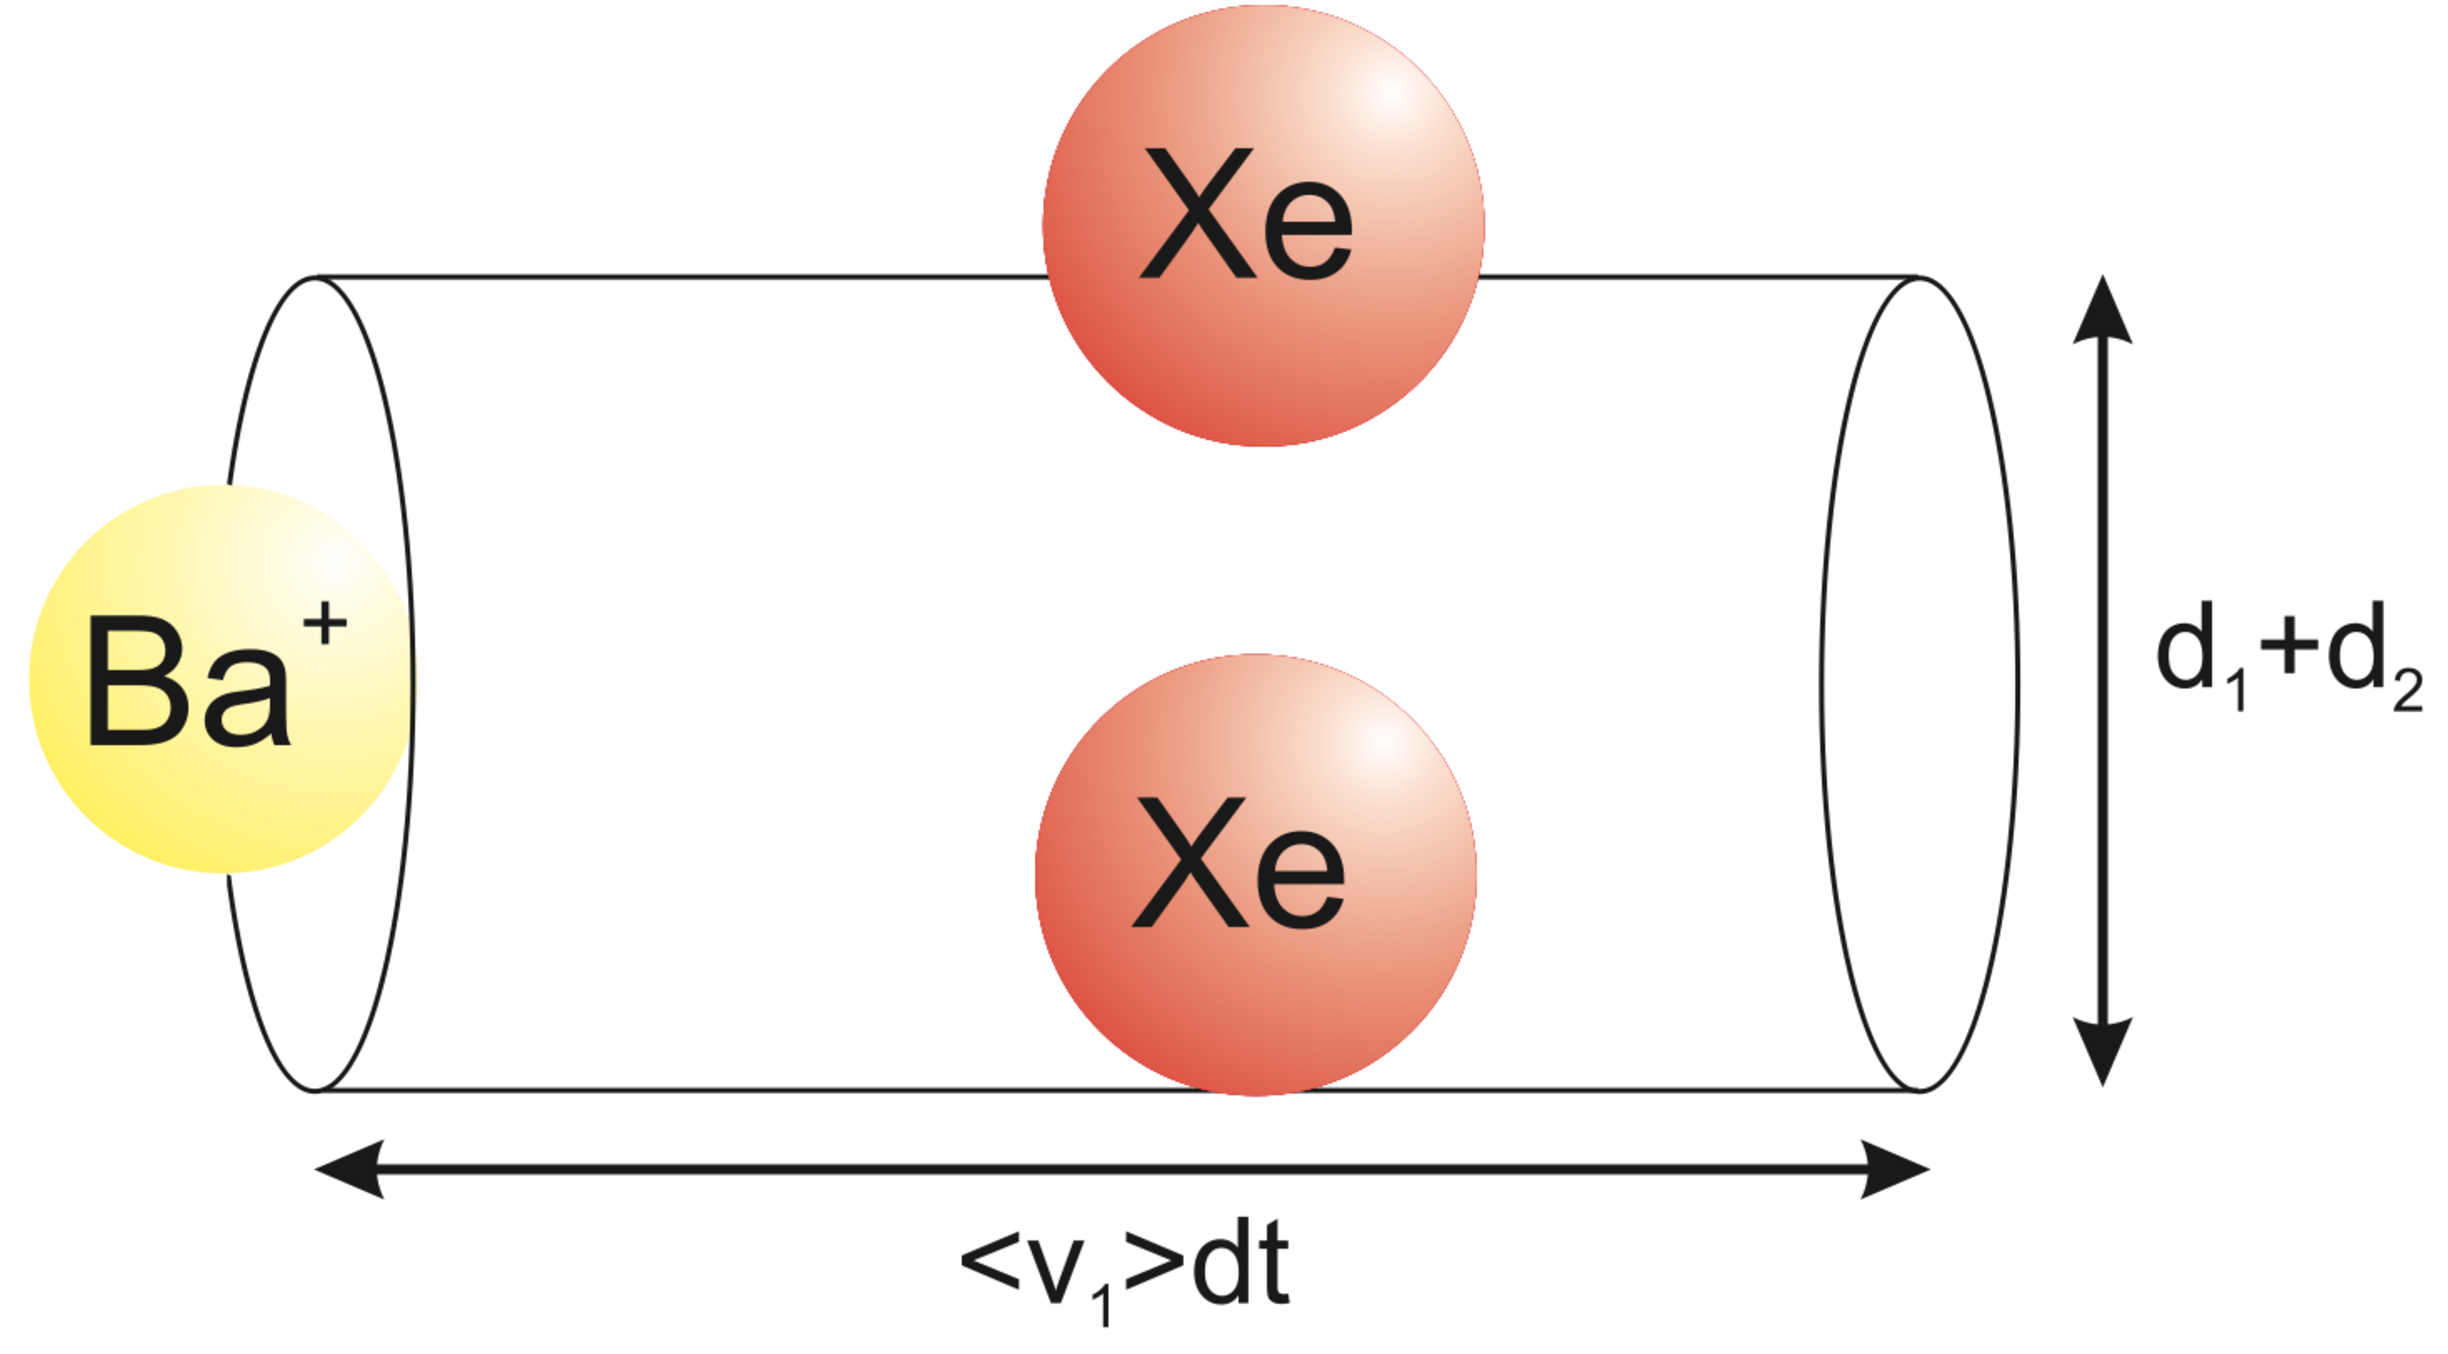
\includegraphics[width=8.3cm, height=4.6cm]{imgs/CylColl.pdf}
\caption{\label{CylColl} Collision volume.}
\end{center}
\end{figure}

According to Fig.\,\ref{CylColl}, for a collision to take place a Xe particle must be inside the cylinder volume defined by:
\begin{align}
& V_{Cyl}=<v_{12}> dt \, \pi \left(\frac{d_1+d_2}{2}\right)^2 \\ \nonumber
& =<v_1> dt \, \pi \left(\frac{d_1+d_2}{2}\right)^2.
\end{align} 
Defining the collision diameter as 
\begin{equation}
d_{12}=\frac{d_1+d_2}{2},
\end{equation}
the number of Xe particles N inside the volume $V_{Cyl}$ (being N$_1$ the total number of Xe atoms) is defined by
\begin{equation}
N=\frac{N_1}{V}V_{Cyl}=\pi d_{12}^2 <v_{1}> dt \frac{N_1}{V},
\end{equation}
and therefore the number of collisions per unit of time is
\begin{equation}
\label{collt}
z=\pi d_{12}^2 <v_{1}>\frac{N_1}{V}.
\end{equation}
If we assume thermodynamic equilibrium, and consider both gases as ideal, we have
\begin{equation}
<v_1>=\left(\frac{8KT}{\pi m_1}\right)^{1/2}
\end{equation}

\begin{equation}
PN_{A}=\frac{N_1}{V}RT,
\end{equation}

being $K$ the Boltzmann constant, $T$ the temperature, $V$ the volume of the vessel of NEXT, $N_A$ the Avogadro constant, and $R$ the ideal gas constant. Substituting these expressions in Eq.\,\ref{collt} we finally obtain

\begin{equation}
\label{collt_2}
z=\pi d_{12}^2  \frac{PN_A}{R T}\left(\frac{8KT}{\pi m_1}\right)^{1/2}.
\end{equation}

The Xe pressure in NEXT will be of around 10\,atm; assuming as well a room temperature of 298\,K, and a diameter of Xe and Ba$^+$ of approximately 2.5$\mathbf{\AA}$, the collision rate can be estimated to be 
\begin{equation}
\label{coll_rate}
z\simeq10^{10}\,\text{s}^{-1}=10\,\text{\ns}.
\end{equation}
 
 Once we know the rate of collisions, we must calculate the number of those collisions that effectively induce a relaxation of the population in the atomic system, i.e., the quenching ratio. Madej and Sankey measured the quenching ratio of the state D$_{5/2}$ of Ba$^+$ ions for different molecules and atoms \cite{Sankey90}. For noble gases they measured a quenching coefficient of 1600$\pm$1300\,s$^{-1}$Pa$^{-1}$ for Ar and 2400$\pm$600\,s$^{-1}$Pa$^{-1}$ for He. Considering that the ionization potential (IP) of Xe is  between the IP for Ar and Xe, we can consider the latter values as the upper and lower limits. Thus, in the conditions of NEXT the quenching rate for Xe, and therefore $\Gamma_{31}$, will be
\begin{equation}
\label{quenching}
1.6\pm1.3\,\text{\ns} \leq z_Q \leq 2.4\pm0.6\,\text{\ns}. 
\end{equation}

According to Eq.\,\ref{quenching} the quenching coefficient for Xe produces a situation of high deshelving of state D ($\Gamma_{31}\gg\Gamma_{21}, \Gamma_{23}$) studied in subsection\,\ref{HighD}. For saturation conditions of the transition S$\rightarrow$P, the rate of fluorescence photons reads
\begin{equation}
\Gamma_{\text{Photons}}\simeq\frac{\Gamma_{31}}{3},
\end{equation}
meaning that there is a generation of the order of 10$^8$ red fluorescence photons per second.

It must be noticed that at high pressure like in NEXT experiment three body collisions, not considered in this simple calculation, must be taken also into account. This will increase the quenching rate, and accordingly the deshelving rate of the D state. 

\subsection{Deshelving induced by a second laser}

In case collisions are not efficient to produce a sufficient deshelving of the D state, one could use instead a second laser either tuned to the P$\leftrightarrow$D or to the D$\leftrightarrow$S transition. 

\begin{figure}[ht!]
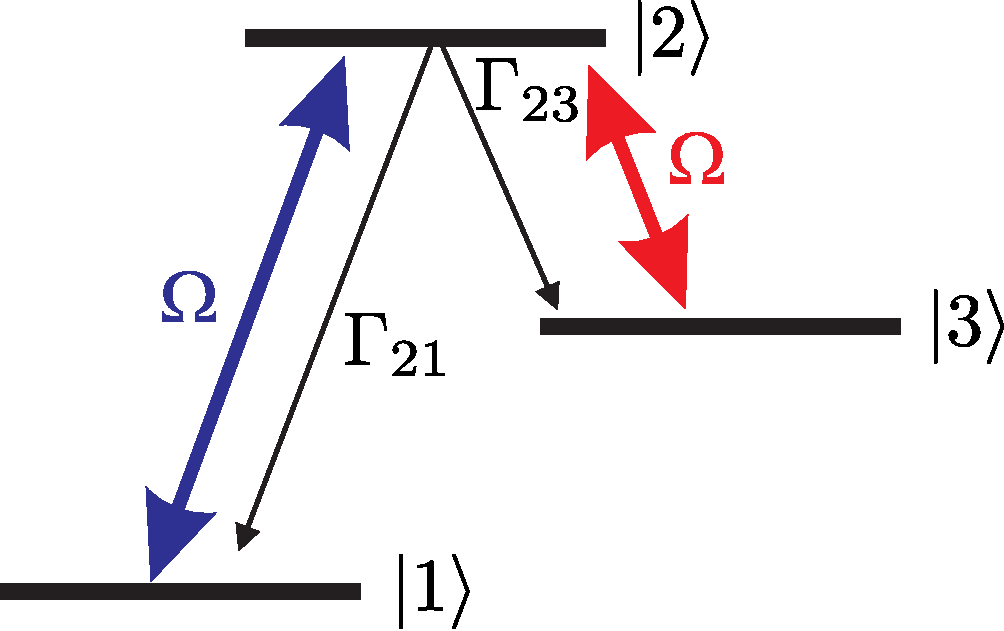
\includegraphics[width=8.3cm, height=5cm]{imgs/levelscheme3.pdf}
\caption{\label{levelscheme3} Level scheme for BaTa with a second laser resonant with the P$\leftrightarrow$D transition.}
\end{figure}

The first possibility is depicted in Fig.\,\ref{levelscheme3}. The main drawback of this choice is that the laser that produces the deshelving has the same photon energy that the fluorescence photons that need to be detected. If the deshelving laser is pulsed, e.g., a few nanoseconds, in principle it would be possible to discriminate between the photons from the laser and from the fluorescence of the P$\rightarrow$D relaxation decay, e.g., synchronizing the photomultipliers with the fluorescence (see Fig.\,\ref{nsDeshelving}). Although this setup is technically feasible it must be noted the collection of the red fluorescence photons will be limited by the repetition rate of  the laser system, i.e., by the number of population cycles that can take place per second which for nanosecond lasers is typically lower than the kHz. Shorter pulse length lasers systems, e.g., femtosecond lasers, have higher repetition rates but they are extremely inefficient coupling bound-bound transitions. This can be easily understood taking into account that for ultrashort pulses the associated bandwidth is much larger than the typical natural bandwidth, i.e., the inverse of radiative lifetime, of atomic states. As a consequence, only a small fraction of the laser bandwidth is effectively on resonance with the transitions, resulting in a very inefficient coupling. 


\begin{figure}[ht!]
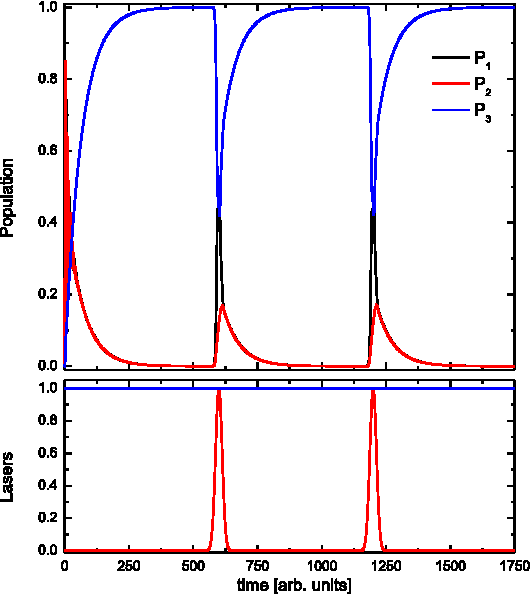
\includegraphics[width=8.3cm, height=9.3cm]{imgs/nsDeshelving.pdf}
\caption{\label{nsDeshelving} A blue CW laser couples the S$\leftrightarrow$P transitions, and a red pulsed laser tuned to the P$\leftrightarrow$D transition deshelves the D state.}
\end{figure}

A second possibility for deshelving the D state is to induce a two photon transition from the state D to the state P (see Fig.\,\ref{levelscheme4}). For a two photon transition the change in the angular moment must be $\Delta L=0,2$ being then the transition D$\leftrightarrow$S allowed. The required wavelength for this laser is around 4.1\,$\mu$m which is not an easily accesible wavelength region for laser systems. In fact , big efforts are being made, see for example \cite{Evans12}, to develope systems capable to cover such energy region because                                    it is not absorbed by the atmosphere (infrared atmospheric window).

\begin{figure}[ht!]
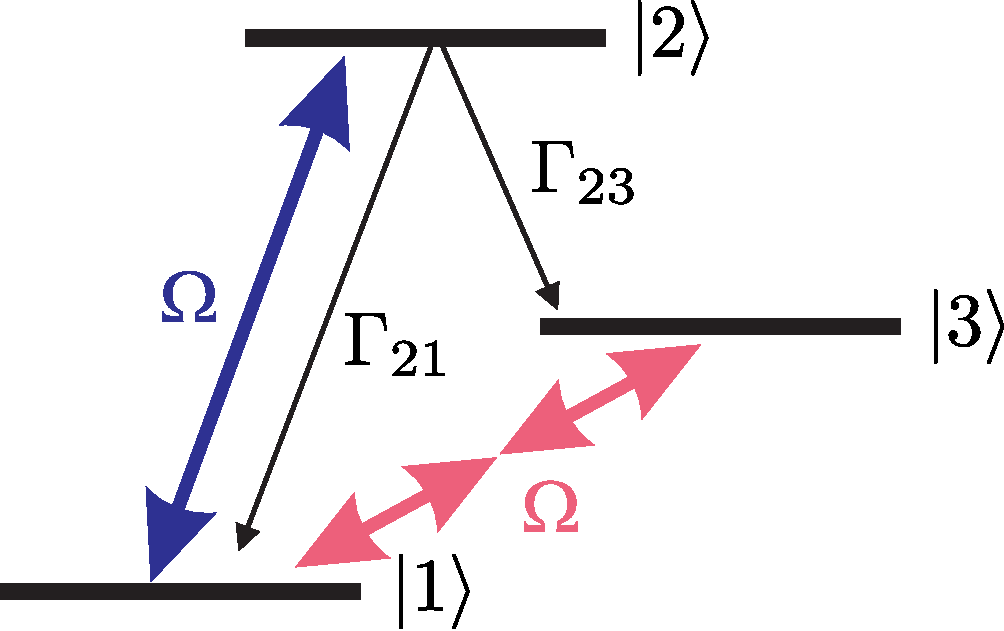
\includegraphics[width=8.3cm, height=5cm]{imgs/levelscheme4.pdf}
\caption{\label{levelscheme4} Level scheme for BaTa with a second laser two photon resonant with the S$\leftrightarrow$D transition.}
\end{figure}

\section{Broadening mechanisms}
For a complete description of BaTa the different broadening mechanisms must be taken into account. These mechanisms not only produce a broadening of the transitions, but also a frequency shift. In order to compensate these effects, the laser that couples the S$\leftrightarrow$P transition needs to be tunable and intense enough to balance the reduction in the absorption cross section produced by the broadening mechanisms.

\subsection{Natural broadening} 
It can be shown that the intensity profile of an absorption line can be written as Lorentzian function \cite{Demtroder03}
\begin{equation}
\label{Lorentz}
I(\omega)\propto\frac{1}{(\omega-\omega_0)^2+\gamma_n^2}
\end{equation}
being $\omega$ the laser frequency, $\omega_0$ the Bohr frequency of the transition, and $\gamma_n$ the natural bandwidth that is equal to:
\begin{equation}
\label{gamma_n}
\gamma_n=1/\tau_{\text{rad.}}
\end{equation}
where $\tau_{\text{rad.}}$ is the radiative lifetime of the chosen transition. The line broadening is 
\begin{equation}
\label{broad_n}
\delta\omega=\gamma_n.
\end{equation}
According to Fig.\,\ref{levelscheme} the state P has two fluorescence decays; therefore, Eq.\,\ref{broad_n} must be modified to
\begin{equation}
\delta\omega=1/\tau_{\text{P}\rightarrow\text{S}}+1/\tau_{\text{P}\rightarrow\text{D}}
\end{equation}
resulting a line broadening of
\begin{equation}
\delta\omega_n=0.13\,\text{\ns} (20.7\,\text{MHz})
\end{equation}

\subsection{Collisional broadening}
If the absorbing atom or molecule is suffering frequent collisions with other particles, the electron energy levels will be distorted. This will produced not only a broadening of the spectral line, collisional or pressure broadening, but also an energy shift of the Bohr transition. Collisions can be either elastic, causing broadening and energy shift, or inelastic causing just broadening. The inelastic collisions are often called quenching collisions because they produce the deshelving of excited states. The collisional mechanisms can be incorporated into Eq.\,\ref{Lorentz} resulting
\begin{equation}
\label{Lorentz2}
I(\omega)\propto\frac{1}{(\omega-\omega_0-\Delta\omega)^2+\gamma^2}
\end{equation}
where $\gamma=\gamma_n+\gamma_{col}$ being $\gamma_{col}$ the total collision rate, and $\Delta\omega=\gamma_{elast}$ the energy shift being $\gamma_{least}$ the rate of elastic collisions. According to rates obtained in Section\,\ref{Subcol}, the collisional energy shift is
\begin{equation}
\Delta\omega\simeq8\,\text{\ns} (1.3\,\text{GHz})
\end{equation}
and the collisional broadening
\begin{equation}
\delta\omega_{coll}\simeq10\,\text{\ns} (1.6\,\text{GHz}).
\end{equation}
It is important to remark that the results obtained in this section are just a first approximation. These values are expected to be much larger when 3 body collisions are taken into account. 

\subsection{Doppler broadening}

The motion of the absorbing atoms produces small variations in the absorption frequency $\omega_0$. The modified absorption frequency reads
\begin{equation}
\omega=\omega_0+\vec{k}\vec{v}.
\end{equation}
According to this equation the absorption frequency shift will be maximum if the particle moves parallel to the laser propagation. Lets assume it propagates in the z direction, then we can write
\begin{equation}
\label{Modfreq}
\omega=\omega_0\left(1+\frac{v_z}{c}\right).
\end{equation}
At thermal equilibrium the particles of a gas follow a Maxwellian velocity distribution defined by
\begin{equation}
\label{Maxwell}
P(v_z)dv_z=\sqrt{\frac{m}{2\pi k_B T}}\text{Exp}\left[-\frac{mv_z^2}{2k_BT}\right]dv_z
\end{equation}
Using Eq.\,\ref{Modfreq} we can modify Eq.\,\ref{Maxwell} and obtain the number of particles with absorption frequencies between $\omega$ and $\omega+d\omega$
\begin{equation}
\label{Maxwell2}
P(\omega)d\omega=\sqrt{\frac{mc^2}{2\pi \omega_0 k_B T}}\text{Exp}\left[-\frac{mc^2}{2k_BT\left(\frac{\omega-\omega_0}{\omega_0}\right)^2}\right]d\omega
\end{equation}
Equation\,\ref{Maxwell2} is a Gaussian distribution with full width at half maximum of
\begin{equation}
\delta\omega_{Doppler}=\left(\frac{\omega_0}{c}\right)\sqrt{8\ln2k_BT/m}
\end{equation}
Assuming room temperature for the Ba$^+$ ions, and provided $\omega_0=3.8\cdot10^{15}$\,s$^{-1}$ the Doppler shift has a value of
\begin{equation}
\delta\omega_{Doppler}\simeq4\,\text{ns}^{-1} (638\,\text{MHz})
\end{equation}

\section{Final considerations}
BLABLABLABLA
\section{Conclusions}
BLBALBAL
\section{Acknowledgments}
BLABLABLA



%
%
%\begin{thebibliography}{7}
%
%\bibitem{Sansonetti10}
%J.E. Sansonetti and J.J Curry, J. Phys. Chem Ref. Data, 39, 4, 2010
%
%\bibitem{Sh90}
%B. W. Shore, The Theory of Coherent Atomic Excitation, Wiley, NY,
%1990.
%
%\bibitem{Sankey90}
%A. A. Madej and J. D. Sankey, Phys. Rev. A, 41, 51, 1990.
%
%\bibitem{Evans12}
%J. W. Evans, P. A. Berry., and K. L. Schepler, Opt.Lett. 37, 23, 2012.
%
%\bibitem{Demtroder03}
%W. Demtr\"oder, Laser spectroscopy. Basic concepts and instrumentation. Springer.
%
%\end{thebibliography}
%
\end{document}

%
%
%%%% CHAPTER 3. ANGEL %%%%%%%%%%%%%%%%%%%
\chapter{Experimental approach: a roadmap} 
\section{Experimental approach}

Study if tagging in situ is possible.

Approach: 

\begin{itemize}
\item identify ion position from kinematical reconstruction in HPXe.
\item Scan barium vertex until barium ion found.
\item Pump with blue laser and if needed with infrared laser.
\item Record red light.
\end{itemize}

\chapter*{Acknowledgements}
This work is supported by the Spanish Secretary of State for Science (SEIDI) under grants CONSOLIDER-INGENIO 2010 CSD2008-0037 (CUP), FPA2012-13697-C04-04, etc.


\bibliographystyle{JHEP}
\bibliography{biblio}

\end{document}
